Hi ha dos problemes bàsics i essencials que han de poder resoldre tots els dispositius. Aquests són: la cerca i l'ordenació. La cerca consisteix a trobar la posició d'una dada en un conjunt. I l'ordenació consisteix a arranjar un conjunt de dades seguint un criteri determinat.

Com tots els problemes hi ha moltes formes de solucionar-los, per això explicaré dos algoritmes per cada problema i els analitzarem per determinar el més eficient.

\section{Cerca}
Aquest problema consisteix a trobar la posició d'una dada en un conjunt. En aquest treball, per simplicitat, utilitzarem un conjunt d'$n$ nombres enters. Per tant, aquest problema té dues entrades: el nombre que cerquem, que anomenarem $k$, i una llista o seqüència d'$n$ nombres. 

Com que la sortida del problema és la posició o índex de $k$ a la llista, hem de definir quin índex té cada nombre. En programació normalment es comença a indexar des de zero, així que el primer element té índex 0, el segon té índex 1 així fins a $n-1$. Per exemple:
\begin{figure}[h]
    \begin{center}
    \renewcommand{\arraystretch}{1.5}
    \begin{tabular}{|c | c | c | c | c |} 
     \hline
     \textit{Llista} & 48 & 5 & 12 & 83 \\ 
     \hline
     Índex & 0 & 1 & 2 & 3 \\
     \hline
    \end{tabular}
    \end{center}
    \caption{Llistes i índexs.}
    \label{fig:my_label}
\end{figure} 

Veiem com la llista té $n = 4$ elements, així que l'últim element té l'índex d'$n-1 = 4-1 = 3$. 

Per exemple, si les entrades d'un problema de cerca són la llista de la figura 2.1, i $k = 5$. Hem de trobar la posició de $k = 5$ en la $Llista = \lbrace 48, 5, 12, 83 \rbrace$. De manera que la sortida seria 1. Ja que la posició de $k = 5$ en la llista té índex = 1. També ho podríem expressar com $Llista_1 = 5$, ja que a l'índex 1 de la llista hi ha l'element 5.

\subsection{Cerca lineal}
L'algoritme de cerca lineal consisteix en mirar cada element un per un i comprovar si coincideixen amb el que estem buscant ($k$). Aquest algoritme acaba quan trobem l'element o hem comprovat tota la llista.

Per exemple, si tenim una $Llista = \lbrace 6, 2, 1, 8, 4 \rbrace$ i $k = 8$. L'algoritme farà el següent:

Anomenem $i$ l'índex del nombre que estem comprovant ($i$ incrementa a cada pas). Així, quan es compleix $Llista_i = k$, la sortida serà igual a $i$.

\begin{enumerate}
    \item Comprova el primer element ($Llista_0 = 6$), com que aquest no és igual a $k = 8$, passa al següent, $i = i + 1$.
    \item $Llista_1 = 2$, com que $2 \neq k$, passa al següent.
    \item Després comprova $i = 2$ com que $Llista_2 \neq k$ comprova el següent.
    \item Finalment $Llista_3 = k$, la sortida és $i = 3$ i acaba l'algoritme.
\end{enumerate}

\newpage
Ho podem representar gràficament amb la figura 2.2.
\begin{figure}[H]
    % \vspace{-18pt}
    \centering
    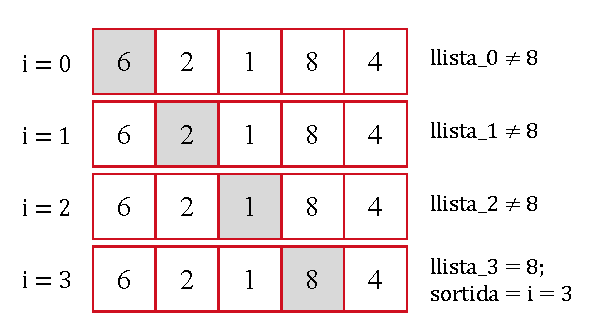
\includegraphics[width=.55\textwidth]{capitols/figures/linearsearch (2).pdf}
    \caption[Exemple. Cerca lineal.]{Exemple. Cerca lineal. Font: elaboració pròpia.}
    \label{fig:my_label}
\end{figure}

Pot passar que l'element no estigui a la llista, en aquest cas comprovaríem els $n$ elements i quan acabés la llista, acabaria l'algoritme.

El pitjor cas possible de la cerca lineal és que l'element se situï en l'última posició o que no hi sigui a la llista. En ambdós casos hauríem d'iterar els $n$ elements, i en cada iteració comprovar si l'element coincideix i si és així assignar l'índex a una variable. Iterar tots els elements suposa $n$ operacions i per cada iteració cal fer 2 operacions. Així que aquest algoritme fa $2n$ operacions i $2n \in O(n)$. Així que aquest algoritme té complexitat lineal. 

Per veure en més detall el funcionament de l'algoritme hi ha una implementació a l'annex 7.3.

\subsection{Cerca dicotòmica}
L'algoritme de la cerca dicotòmica resol el mateix problema que la cerca lineal, però amb el requisit que la llista ha d'estar ordenada. Aquest algoritme és el mateix que el de l'exemple del diccionari de la complexitat logarítmica. 

Aquest algoritme consisteix a acotar el rang on podem trobar l'element fins que només en queda un i coincideix amb el que busquem. Per acotar el rang partim la llista per la meitat, i com que està ordenada, podem saber en quina meitat es troba $k$, de manera que a cada pas podem descartar la meitat dels elements que ens quedaven.

\newpage
Per exemple, si tenim la $Llista = \lbrace 2, 4, 7, 12, 24, 38, 51, 56, 62, 65, 71, 83, 89, 98, 99 \rbrace$, $n = 15$ i $k = 62$. L'algoritme fa el següent:

\begin{enumerate}
\item $k$ es troba en el rang 0 - 14 ambdós inclosos, per tant,  calculem en quin índex queda la dada central, així, $\frac{0+14}{2} = 7$. Com que $k$ és més gran que la dada de l'índex 7, podem descartar totes les posicions més petites a l'índex 7 inclòs. És a dir, com que $Llista_7 = 56 < k$  podem assegurar que $k$ es troba en el rang 8 - 14 ambdós inclosos.
\item Repetim el pas 1 però en el rang 8 - 14 ambdós inclosos. La dada central es troba a l'índex $\frac{8+14}{2} = 11$. Com que $Llista_{11} = 83 > k$, $k$ es troba a l'esquerra de l'índex 11, en el rang 8 - 10 ambdós inclosos. 
\item Trobem la dada central de 8 - 10, $\frac{8+10}{2} = 9$, $Llista_9 = 65 > k$ . Per tant, $k$ es troba en el rang 8 - 8.
\item La dada central de 8 - 8 es troba en $\frac{8+8}{2} = 8$, $Llista_8 = 62 = k$. Per tant, acaba l'algoritme i la sortida és 8. 
\end{enumerate}

Ho representem en la figura 2.3. Els elements en verd representen els que no han estat descartats, els que estan en blau representen les dades centrals, i en vermell representen $k$.
% \vspace{18pt}
\begin{figure}[H]
    \centering
    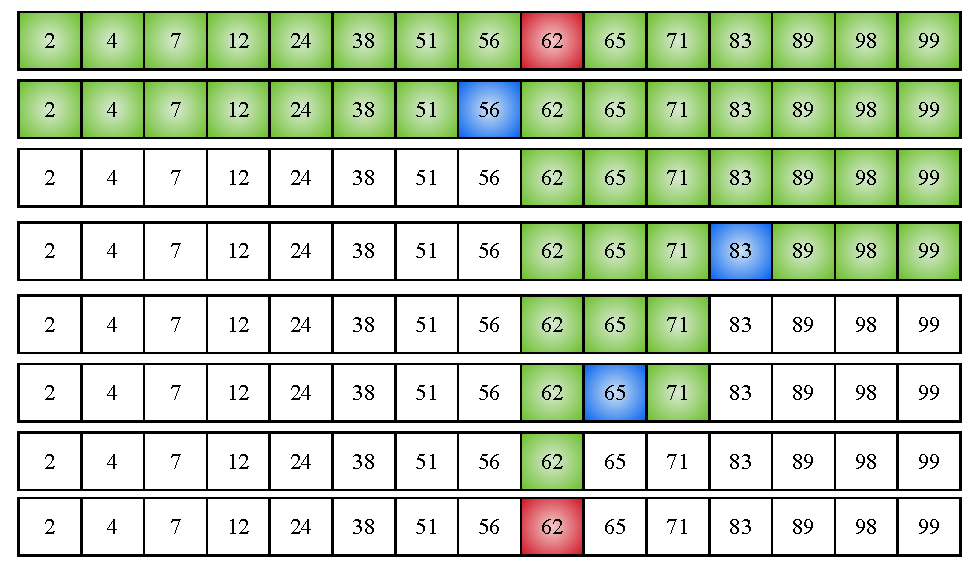
\includegraphics[width=.7\textwidth]{capitols/figures/binary2.pdf}
    \caption[Exemple. Cerca dicotòmica.]{Exemple. Cerca dicotòmica. Font: elaboració pròpia.}
    \label{fig:my_label}
\end{figure}
\vspace{-18pt}

El pitjor cas possible és que $k$ no es trobi a la llista, ja que hauríem d'arribar a dividir les dades d'una en una per assegurar-nos que no hi estigui. Això també ha passat en l'exemple de la figura 2.3, encara que $k$ estigués a la llista. En canvi, si haguéssim escollit $k = 83$, hauríem acabat l'algoritme partint les dades una sola vegada.

Com hem explicat al punt 1.2.2, aquest algoritme té complexitat logarítmica, ja que $\lceil\log_2{n}\rceil$ és la quantitat necessària de passos per partir les dades de la manera com ho fa la cerca dicotòmica. En la figura 1.7 es pot veure com es parteixen les dades igual que en aquest algoritme, i la relació que té amb els logaritmes.

Com hem vist, a cada iteració s'ha de buscar la dada central i en el pitjor dels casos fer tres comparacions (si $Llista_i = k, Llista_i > k, Llista_i < k$) i retornar l'índex. Així que més concretament aquest algoritme fa $\log_2{n} \cdot 5$ operacions. Com que $5 \cdot \log_2{n} \in O(\log_2{n})$ aquest algoritme té complexitat logarítmica.

Per veure en més detall el funcionament de l'algoritme hi ha la implementació a l'annex 7.4.

\section{Ordenació}
En aquest treball ordenarem ascendentment una llista de nombres enters. L'entrada d'aquest problema és una llista d'$n$ elements. I la sortida consisteix en els $n$ elements ordenats ascendentment.

Hi ha molts algoritmes diferents per resoldre aquest problema, i tots tenen avantatges i inconvenients. En aquest treball ens centrem només en l'eficiència temporal, però hi ha molts altres factors que també afecten l'eficiència de l'algoritme i depenent de la situació cal tenir-ho en compte. N'hi ha que són molt eficients temporalment, però ocupen molta memòria, en canvi, n'hi ha que tenen una menor eficiència temporal, però ocupen menys memòria. N'hi ha que són més convenients si hi ha moltes dades repetides, n'hi ha que són específics per a estructures de dades determinades (llistes, grafs, heaps...).

\subsection{Ordenació de bombolla}
Aquest algoritme consisteix a intercanviar dos elements adjacents si no estan en ordre.

Per exemple, si tenim una $Llista = \lbrace7, 2, 5, 3, 11\rbrace$ i $n = 5$, l'algoritme farà el següent:

\begin{enumerate}
    \item Comprova el primer i segon element (7 i 2), com que $7 > 2$ els intercanvia. I ens queda $Llista = \lbrace2, 7, 5, 3, 11\rbrace$.
    \item Comprova el segon i tercer element. Com que $7 > 5$, els intercanvia. I queda $Llista = \lbrace2, 5, 7, 3, 11\rbrace$.
    \item Comprova el tercer i quart element. Com que $7 > 3$, els intercanvia. I queda $Llista = \lbrace2, 5, 3, 7, 11\rbrace$.
    \item Comprova el quart i cinquè element. Com que $7 < 11$, no els intercanvia. I la llista queda igual $Llista = \lbrace2, 5, 3, 7, 11\rbrace$.
    \item Ara ja ha acabat la llista, i ha de repetir el mateix procediment $n$ vegades en total. \\ Comprova el primer i segon element. Com que $2 < 5$, queden igual. I queda $Llista = \lbrace2, 5, 3, 7, 11\rbrace$.
    \item Comprova el segon i tercer element. Com que $5 > 3$, els intercanvia. I queda $Llista = \lbrace2, 3, 5, 7, 11\rbrace$.
    \item Ara la llista ja està ordenada, però els ordinadors no ho poden saber si no ho comproven. I no ho comproven perquè això faria l'algoritme poc eficient, ja que cada comprovació té complexitat lineal\footnote{Per comprovar que la llista ha quedat ordenada, caldria iterar una vegada els $n$ elements i comprovar que l'element actual és més petit al següent. Aquest procediment té un cost lineal $O(n)$}. Això comporta que en un ordinador aquest algoritme segueixi funcionant fins a repetir aquest procés un total d'$n$ vegades, encara que no es canviarà d'ordre cap dada. De manera que no hi ha un pitjor cas possible, ja que en tots els casos es farà la mateixa quantitat d'operacions.
\end{enumerate}

Aquest algoritme repeteix $n$ vegades el mateix procediment. Aquest procediment itera fins a $n-1$ i a cada iteració fa tres operacions per intercanviar dos elements. Per tant, l'ordenació de bombolla té una complexitat d'$n \cdot (n-1) \cdot 3 = 3n^2 - 3n \in O(n^2)$. Per això aquest algoritme té complexitat quadràtica.

Per veure en més detall el funcionament de l'algoritme hi ha la implementació a l'annex 7.5.

\subsection{Ordenació per barreja} %merge
El funcionament d'aquest algoritme el podríem separar en dues parts: en la primera part divideix les dades igual que en la cerca dicotòmica (figura 2.4), i en la segona part les uneix fins que queden en una sola llista ordenada (figura 2.5).

\begin{figure}[H]
    \centering
    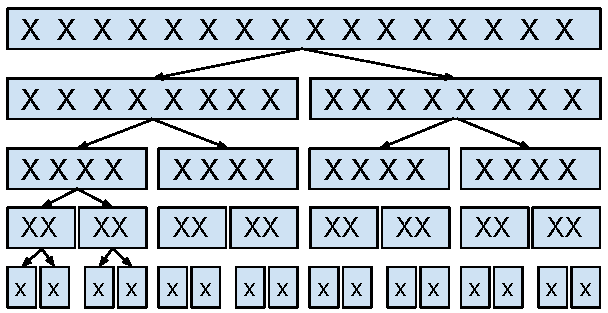
\includegraphics[width=.6\textwidth]{capitols/figures/merge.pdf}
    \caption[Divisió de les dades.]{Divisió de les dades. Font: elaboració pròpia.}
    \label{fig:my_label}
\end{figure}
\vspace{-.8cm}
En la figura 2.4 podem veure com cada llista es divideix per la meitat fins a quedar dades individuals. Igual que en la cerca dicotòmica, i, per tant, també té complexitat logarítmica.
% \vspace{-.5cm}
\begin{figure}[H]
    \centering
    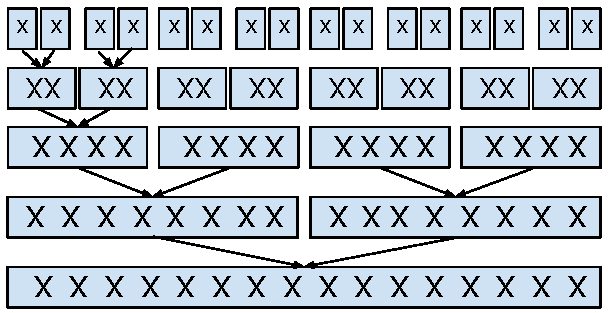
\includegraphics[width=.6\textwidth]{capitols/figures/merge2.pdf}
    \caption[Unir les dades.]{Unir les dades. Font: elaboració pròpia.}
    \label{fig:my_label}
\end{figure}
\vspace{-.5cm}
\begin{wrapfigure}[10]{R}{.35\textwidth}
\vspace{-18pt}
    \centering
    \includegraphics[width=.35\textwidth]{capitols/figures/Còpia de merge2.pdf}
    \caption[Exemple d'unió les dades.]{Exemple d'unió de les dades. Font: elaboració pròpia.}
    \label{fig:my_label}
\end{wrapfigure}
Unir les dades és molt simple. Com que comencem amb dades individuals sempre són grups de dades ordenades, per això les podem ordenar tan ràpidament. Primer mirem la dada més petita dels dos grups que volem unir, és a dir, la primera. Després posem la més petita de les dues a la següent llista i avancem una posició a la llista d'on hem tret la dada. Ho podem representar gràficament amb la figura 2.6.

Aquest procediment es repeteix cada vegada que s'ajunten dues llistes.

Podem posar un exemple d'aquest algoritme per a $n = 8$ i $Llista = \lbrace5, 2, 4, 7, 1, 3, 2, 6\rbrace$ en la figura 2.7.
% \vspace{18pt}
\begin{figure}[H]
    \centering
    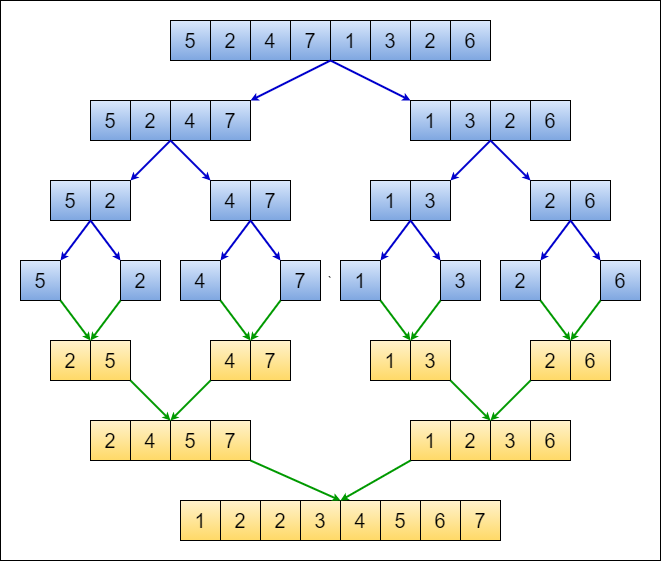
\includegraphics[width=.55\textwidth]{capitols/figures/merge5.png}
    \vspace{10pt}
    \caption[Exemple d'ordenació per barreja.]{Exemple d'ordenació per barreja. Font: https://levelup.gitconnected.com/visualizing-designing-and-analyzing-the-merge-sort-algorithm-cf17e3f0371f.}
    \label{fig:my_label}
\end{figure}

\vspace{-18pt}
En la primera part de l'algoritme (part blava) només es parteixen les dades, i en la segona part (part groga) s'ajunten com hem vist a la figura 2.6 fins a obtenir una única llista.

Analitzarem la complexitat d'aquest algoritme separant la part blava de la groga, i després sumarem els dos resultats. La part blava com ja hem vist anteriorment té complexitat logarítmica. I la part groga té complexitat $O(n \cdot log_2{n})$.

En la figura 2.6 hem ajuntat dues llistes de 3 elements per obtenir una llista d'$n = 6$, i hem fet $n$ operacions, ja que hem recorregut cada llista una vegada. De manera que el procediment d'ajuntar dues llistes té complexitat lineal.

En la part groga de la figura 2.7 hi ha les mateixes particions que en la part blava però invertides. És a dir, hi ha $\log_2{n}$ passos a la part groga, i a cada pas ajuntem els $n$ elements de forma lineal. Els ajuntem en llistes diferents de mides diferents, però la suma d'aquestes subllistes tenen mida $n$. Així que en total fem un procediment lineal $\log_2{n}$ vegades, $O(n \cdot \log_2{n})$.

Si ho ajuntem tot ens queda una complexitat de $O(\log_2{n}) + O(n \cdot \log_2{n} ) = O(\log_2{n} + n \cdot \log_2{n}) = O(n \cdot \log_2{n})$, ja que en l'últim pas podem eliminar el primer $\log_2{n}$ ja que és un terme de creixement més lent (propietat 2).

Per veure en més detall el funcionament de l'algoritme hi ha la implementació a l'annex 7.6.
